\chapter{실험}\label{chap:experiments}

이 장에서는 VLM에 영상을 입력하면서 프레임마다 읽을 행을 선택하고, 영상에 대한 질문의 \textbf{정확도}와 선택한 행을 SSD에서 읽는 \textbf{프레임당 시간}을 측정한다. \ref{sec:exp-setup}절은 모델과 자료, 선택 방법의 설정을, \ref{sec:exp-measure}절은 측정 방법을, \ref{sec:exp-results}절은 결과를 다룬다. \ref{sec:exp-paper}절에서는 정확도를 Neuron Chunking 논문의 값과 비교한다.

모든 측정은 표~\ref{tab:environment}의 Jetson Orin Nano 한 대에서 수행하였다. 보드의 종류와 SSD의 모델은 Neuron Chunking이 기본 장치로 사용한 구성과 같다 \cite{yang2025}.

\begin{table}[htbp]
    \centering
    \caption{실험 장치}
    \label{tab:environment}
    \begin{tabular}{ll}
        \toprule
        항목 & 사양 \\
        \midrule
        기기 & NVIDIA Jetson Orin Nano Developer Kit (모듈 P3767-0005) \\
        CPU & Arm Cortex-A78AE (6코어) \\
        메모리 & 7.4 GiB, CPU와 GPU가 공유 \\
        GPU & 내장 Orin GPU \\
        SSD & SK hynix Gold P31 500 GB (NVMe, PCIe 3.0 x4) \\
        파일 시스템 & ext4, I/O 스케줄러 \texttt{none} \\
        운영체제 & Ubuntu 22.04.5, Jetson Linux R36.4.4 (kernel 5.15.148) \\
        전원 설정 & \texttt{MAXN\_SUPER} 모드, CPU 클럭 1.728 GHz 고정 \\
        \bottomrule
    \end{tabular}
\end{table}

\section{실험 설정}\label{sec:exp-setup}

\subsection{모델과 평가 자료}\label{sec:exp-model}

모델은 Neuron Chunking이 평가한 모델 중 하나인 LLaVA-OneVision-Qwen2-0.5B\footnote{\url{https://huggingface.co/llava-hf/llava-onevision-qwen2-0.5b-ov-hf}}이다. 행을 선택하는 대상은 언어 모델의 projection 168개이며, block마다 다음 일곱 개가 있다.

\begin{itemize}
\item Attention: \texttt{q\_proj}, \texttt{k\_proj}, \texttt{v\_proj}, \texttt{o\_proj}
\item MLP: \texttt{gate\_proj}, \texttt{up\_proj}, \texttt{down\_proj}
\end{itemize}

가중치는 원소당 2바이트이므로, 행당 원소 수가 $D$인 projection에서 한 행의 크기는 $w=2D/1024$ KiB이다.

평가 자료는 Neuron Chunking이 사용한 TempCompass\footnote{\url{https://huggingface.co/datasets/lmms-lab/TempCompass}}의 객관식 질문이다. 410개 영상 가운데 무작위로 고른 100개 영상의 질문 391개를 평가에 사용하고, 나머지 영상 중 25개를 calibration에 사용하였다. 영상마다 균등한 간격으로 32개 프레임을 뽑았으며, 프레임 하나는 토큰 196개가 된다.

\subsection{읽기 비용의 측정}\label{sec:exp-cost}

\ref{sec:chunk-cost}절의 구간 읽기 비용은 이 장치의 SSD에서 측정하였다. SSD에 저장한 128 MiB 파일을 대상으로 6개 스레드와 O\_DIRECT를 사용하였고, 요청 크기는 다음 두 구간의 432개이다.

\begin{itemize}
\item 1--320 KiB: 1 KiB 간격
\item 324--768 KiB: 4 KiB 간격
\end{itemize}

전체 크기 범위를 7회 반복하여 측정하고, 크기마다 7회의 중앙값을 그 크기의 읽기 비용으로 삼았다. 측정 절차는 선행 연구 \cite{seol2026}와 같다. Paper와 Tiles에는 모두 이 값을 $T$로 주었다. 측정한 크기 가운데 KiB당 비용이 가장 작은 크기는
\[
z_\ast=648\ \mathrm{KiB}
\]
였다.

\subsection{순서와 예산의 계산}\label{sec:exp-calibration}

Calibration 영상 25개로 \ref{sec:hot-cold}절의 순서와 \ref{sec:budgets}절의 예산을 계산하였다. 두 값은 추론 전에 한 번 구해 두는 것이므로 별도의 노트북 컴퓨터에서 계산하였고, Jetson에서는 그 결과를 그대로 사용하였다.

\begin{itemize}
\item \textbf{Hot--cold 순서}: Calibration 영상의 프레임을 하나씩 언어 모델에 입력하고, 프레임 하나를 \ref{sec:hot-cold-order}절의 입력 하나로 삼았다. Projection마다 $E=800$개 입력에서 활성 횟수를 세어 순열을 구하였다.
\item \textbf{행 예산}: 오차는 calibration 영상마다 가운데 프레임 하나씩, 25개 프레임에서 측정하였다. 기준 projection은 \texttt{q\_proj}이고 그 간격은 $\alpha=0.05$이다. 요청 비율은 $f\in\{0.3,0.5,0.7\}$의 세 가지이다.
\end{itemize}

표~\ref{tab:projections}\는 projection별 크기와 탐색 간격, 그리고 탐색으로 얻은 예산이다. 간격 $\delta_p$는 projection에 따라 0.0092에서 0.35까지 다르지만, 어느 projection에서든 한 단계는 block 하나의 projection 가중치 가운데 0.27\%를 덜 읽게 한다.

\begin{table}[htbp]
    \centering
    \caption{Projection별 크기와 탐색 간격, 읽는 행의 비율 $R_p/N_p$ (24개 block의 평균)}
    \label{tab:projections}
    \begin{tabular}{llrrrr}
        \toprule
        & & & \multicolumn{3}{c}{읽는 행의 비율 (\%)} \\
        \cmidrule(lr){4-6}
        Projection & $N_p\times D_p$ & $\delta_p$ & $f=0.3$ & $f=0.5$ & $f=0.7$ \\
        \midrule
        \texttt{q\_proj} & $896\times896$ & 0.05 & 22.6 & 26.8 & 36.4 \\
        \texttt{k\_proj} & $896\times128$ & 0.35 & 47.4 & 59.1 & 66.4 \\
        \texttt{v\_proj} & $896\times128$ & 0.35 & 76.6 & 81.0 & 86.9 \\
        \texttt{o\_proj} & $896\times896$ & 0.05 & 34.5 & 41.6 & 51.4 \\
        \texttt{gate\_proj} & $896\times4864$ & 0.0092 & 25.7 & 47.4 & 68.7 \\
        \texttt{up\_proj} & $896\times4864$ & 0.0092 & 40.1 & 66.0 & 86.6 \\
        \texttt{down\_proj} & $4864\times896$ & 0.0092 & 22.0 & 41.0 & 63.3 \\
        \bottomrule
    \end{tabular}
\end{table}

이렇게 정한 예산은 projection마다 크게 다르다. $f=0.5$에서 \texttt{q\_proj}는 행의 26.8\%를, \texttt{v\_proj}는 81.0\%를 읽는다. 세 요청 비율에서 모델이 읽는 가중치는 전체 projection 가중치의 29.7\%, 49.9\%, 69.8\%이다.

\subsection{선택 방법의 설정}\label{sec:exp-methods}

비교한 방법은 다음 네 가지이다.

\begin{itemize}
\item \textbf{Dense}: 모든 행을 읽는다.
\item \textbf{Top-$R$}: 중요도가 가장 큰 $R_p$개 행을 선택한다. Neuron Chunking이 기준으로 삼은 방법이며, 논문과 같이 행을 원래 순서로 저장한다. CPU에서 PyTorch의 정렬로 실행한다.
\item \textbf{Paper}: \ref{sec:paper-greedy}절의 방법이다. Hot--cold 순서로 저장한 행에서 선택한다. 원 논문의 공개 구현을 사용하였으며, 후보의 점수를 GPU에서 정렬한다.
\item \textbf{Tiles}: \ref{sec:tiles}절의 방법이다. Hot--cold 순서로 저장한 행에서 선택한다. CPU에서 실행하는 C++ 구현이다.
\end{itemize}

같은 projection과 요청 비율에서 세 선택 방법은 같은 예산 $R_p$를 받는다. Tiles의 타일 길이와 Paper의 후보 설정은 projection의 크기에 따라 표~\ref{tab:selector-settings}\와 같이 정하였다.

\begin{table}[htbp]
    \centering
    \caption{Projection의 크기별 Tiles와 Paper의 설정}
    \label{tab:selector-settings}
    \begin{tabular}{lrrrr}
        \toprule
        $N\times D$ & $w$ (KiB) & Tiles의 $B$ (행) & Paper의 $\ell_{\min}$ (KiB) & Paper의 $J$ (KiB) \\
        \midrule
        $896\times128$ & 0.25 & 2592 & 4 & 4 \\
        $896\times896$ & 1.75 & 371 & 8 & 8 \\
        $896\times4864$ & 9.50 & 69 & 4 & 20 \\
        $4864\times896$ & 1.75 & 371 & 12 & 20 \\
        \bottomrule
    \end{tabular}
\end{table}

\textbf{Tiles}의 타일 길이는 $B=\lceil648/w\rceil$이다. $896\times128$인 \texttt{k\_proj}와 \texttt{v\_proj}에서는 $B$가 행 수 $N$보다 크므로, Tiles는 항상 길이 $R_p$의 구간 하나를 선택한다.

\textbf{Paper}의 $\ell_{\min}$과 $J$는 측정 전에 크기마다 다음 순서로 정하였다. 최대 후보 길이 $\ell_{\max}$는 읽기 비용을 측정한 가장 큰 크기인 768 KiB에 해당하는 행 수이다.

\begin{enumerate}
\item 두 값을 각각 4--64 KiB 범위에서 4 KiB 간격으로 바꾸어 가며, 난수 중요도에서 선택 시간을 측정한다.
\item 선택 시간이 1.6 ms 이하인 설정 가운데 두 값의 합이 가장 작은 것을 고른다.
\end{enumerate}

\section{측정 방법}\label{sec:exp-measure}

\subsection{추론 과정}\label{sec:exp-inference}

언어 모델은 영상 앞의 텍스트를 읽은 뒤 프레임을 한 번에 하나씩 읽는다. 논문의 공개 구현과 같이 프레임을 읽을 때에만 행을 선택하고, 텍스트를 읽을 때에는 모든 행을 사용한다. 프레임 하나를 읽을 때 각 projection은 다음을 수행한다.

\begin{enumerate}
\item 입력 activation에서 행의 중요도를 계산하고, 저장 순서에 맞추어 나열한다.
\item 선택 방법으로 예산 $R_p$ 안에서 읽을 행의 mask를 구성한다.
\item 선택되지 않은 행에 대응하는 입력 채널을 0으로 둔다.
\end{enumerate}

\ref{sec:sparsification}절에서 보았듯이 3의 결과는 선택한 행만 읽어 계산한 값과 같다. 정확도는 이 방식으로 모든 가중치를 메모리에 둔 채 측정하고, 읽기 시간은 선택된 행을 SSD의 파일에서 읽어 따로 측정하였다.

\subsection{정확도}\label{sec:exp-accuracy}

\textbf{정확도}는 391개 질문 중 맞게 답한 비율이다. 질문 뒤에 선택지 하나를 고르라는 지시를 붙이고, 답의 첫 위치에서 logit이 가장 큰 선택지 문자를 모델의 답으로 삼았다. 95\% 신뢰구간은 10,000회 재표집한 BCa bootstrap으로 구하였다.

모든 조건이 같은 질문에 답하므로, 두 조건을 비교할 때에는 질문끼리 짝지은 차이를 사용하였다. 질문마다 두 조건의 정답 여부의 차이를 구하고, 그 평균과 신뢰구간을 같은 방법으로 계산하였다.

\subsection{프레임당 시간}\label{sec:exp-time}

\textbf{프레임당 시간}은 평가 영상 하나에서 측정하였다. Projection마다 가중치를 파일 하나로 SSD에 저장하되, 원래 순서와 hot--cold 순서로 각각 저장하였다. 프레임을 읽을 때마다, 그 프레임에서 선택된 행을 방법의 저장 순서에 해당하는 파일에서 읽었다. 읽기에는 6개 스레드와 O\_DIRECT를 사용하였고, 768 KiB를 넘는 요청은 나누어 읽는다. 처음 2개 프레임은 warmup으로 두고, 나머지 30개 프레임에서 표~\ref{tab:times}의 시간을 기록하였다.

\begin{table}[htbp]
    \centering
    \caption{프레임마다 기록한 시간}
    \label{tab:times}
    \begin{tabular}{ll}
        \toprule
        시간 & 측정 범위 \\
        \midrule
        \textbf{선택 시간} & 중요도에서 mask를 구성하는 시간을 모든 projection에 대해 더한 값 \\
        \textbf{읽기 시간} & 선택된 행을 읽는 시간을 모든 projection에 대해 더한 값 \\
        \textbf{로딩 시간} & 선택 시간과 읽기 시간의 합 \\
        \bottomrule
    \end{tabular}
\end{table}

결과에는 30개 프레임의 중앙값을 사용한다. 로딩 시간은 프레임마다 두 시간을 더한 뒤 중앙값을 구한 것이므로, 두 중앙값을 더한 값과 조금 다를 수 있다. 중요도를 계산하는 시간과 모델의 연산 시간은 어느 시간에도 들어 있지 않다.

이 장치에서는 읽기 하나가 커널의 I/O timeout까지 멈추는 일이 드물게 있었다. 500 ms 이상 걸린 읽기는 버리고 다시 읽었으며, 이 측정에서 버린 읽기는 20회이다.

\section{정확도와 프레임당 시간}\label{sec:exp-results}

그림~\ref{fig:accuracy-latency}\은 조건별 정확도와 프레임당 시간이다. 왼쪽 패널의 가로축은 읽기 시간이고, 오른쪽 패널의 가로축은 로딩 시간이다. 점 옆의 숫자는 요청 비율이며, 점선은 Dense의 위치에서 교차한다. 세로 점선의 오른쪽에 있는 조건은 모든 행을 읽는 것보다 오래 걸린다. 표~\ref{tab:summary}\는 같은 결과의 수치이다.

\begin{figure}[htbp]
    \centering
    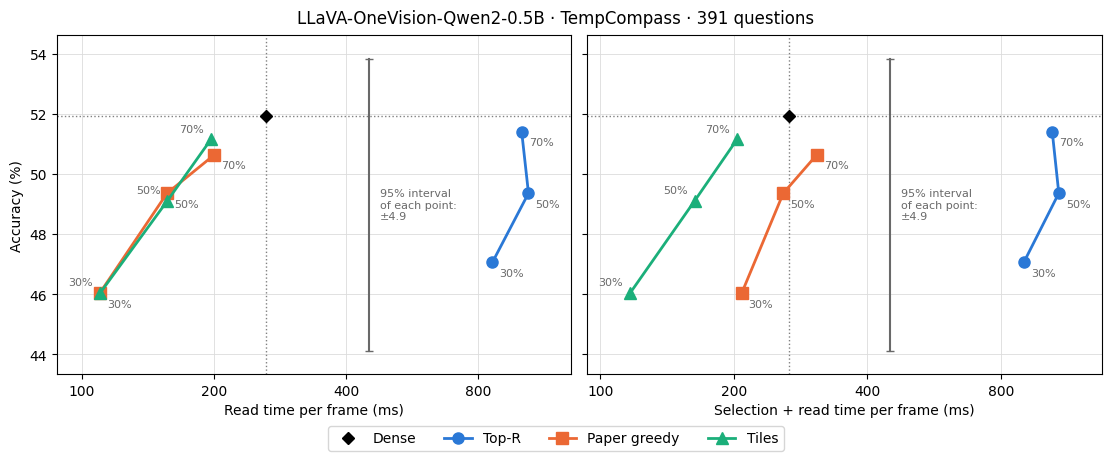
\includegraphics[width=\textwidth]{figures/05/01_accuracy_latency.png}
    \caption{정확도와 프레임당 시간. 가로축은 로그 척도이다. 회색 막대는 정확도의 95\% 신뢰구간 하나를 척도로 나타낸 것이며, 그림의 Paper greedy는 본문의 Paper이다.}
    \label{fig:accuracy-latency}
\end{figure}

\begin{table}[htbp]
    \centering
    \caption{조건별 정확도와 프레임당 시간 (30개 프레임의 중앙값). Dense의 선택 시간은 모든 행을 선택하는 mask를 만드는 시간이다.}
    \label{tab:summary}
    \setlength{\tabcolsep}{5pt}
    \begin{tabular}{lrrrrr}
        \toprule
        방법 & $f$ & 정확도 (\%) [95\% 구간] & 선택 시간 (ms) & 읽기 시간 (ms) & 로딩 시간 (ms) \\
        \midrule
        Dense & 1.0 & 51.9 [47.1, 56.8] & 4.3 & 262.0 & 266.3 \\
        \midrule
        Top-$R$ & 0.3 & 47.1 [42.2, 51.9] & 40.4 & 861.5 & 902.0 \\
                & 0.5 & 49.4 [44.5, 54.2] & 40.6 & 1041.1 & 1081.6 \\
                & 0.7 & 51.4 [46.5, 56.3] & 40.8 & 1004.6 & 1045.5 \\
        \midrule
        Paper & 0.3 & 46.0 [41.2, 50.9] & 98.6 & 109.7 & 208.5 \\
              & 0.5 & 49.4 [44.5, 54.2] & 102.2 & 156.2 & 258.7 \\
              & 0.7 & 50.6 [45.8, 55.5] & 106.5 & 200.1 & 307.8 \\
        \midrule
        Tiles & 0.3 & 46.0 [41.2, 50.9] & 6.9 & 109.9 & 116.8 \\
              & 0.5 & 49.1 [44.2, 54.0] & 6.9 & 156.4 & 163.2 \\
              & 0.7 & 51.2 [46.3, 56.0] & 6.8 & 196.6 & 203.4 \\
        \bottomrule
    \end{tabular}
\end{table}

\textbf{정확도}는 같은 요청 비율에서 방법 사이에 구별되지 않았다. 정확도의 95\% 신뢰구간은 모든 조건에서 폭이 9.7\%p인데, 같은 $f$에서 세 방법의 정확도는 약 1\%p 안에 모여 있다. 표~\ref{tab:paired}\는 같은 질문끼리 짝지은 차이이다. Tiles와 Paper의 차이는 세 비율에서 최대 0.5\%p이며, 아홉 개의 신뢰구간이 모두 0을 포함한다.

\begin{table}[htbp]
    \centering
    \caption{같은 요청 비율에서 두 방법의 정확도 차이 (\%p) [95\% 구간]}
    \label{tab:paired}
    \begin{tabular}{lrrr}
        \toprule
        비교 & $f=0.3$ & $f=0.5$ & $f=0.7$ \\
        \midrule
        Tiles $-$ Paper & $0.0$ [$-2.3$, $2.3$] & $-0.3$ [$-2.8$, $2.3$] & $0.5$ [$-1.0$, $2.3$] \\
        Tiles $-$ Top-$R$ & $-1.0$ [$-4.1$, $2.0$] & $-0.3$ [$-3.1$, $2.6$] & $-0.3$ [$-1.5$, $1.0$] \\
        Paper $-$ Top-$R$ & $-1.0$ [$-3.8$, $1.8$] & $0.0$ [$-2.6$, $2.6$] & $-0.8$ [$-2.8$, $1.0$] \\
        \bottomrule
    \end{tabular}
\end{table}

읽는 가중치가 줄면 정확도는 낮아진다. Dense의 정확도는 51.9\%이고, $f=0.3$에서는 세 방법 모두 46.0--47.1\%이다. 이 비율에서는 세 방법 모두 Dense와 짝지은 차이의 신뢰구간이 0보다 아래에 있었다.

\textbf{읽기 시간}에서는 Top-$R$만 Dense보다 길었다. Top-$R$은 행의 일부만 읽는데도 861.5--1041.1 ms가 걸려, 모든 행을 읽는 262.0 ms의 3.3--4.0배이다. 행의 연속성을 고려하지 않는 선택이 전체를 읽는 것보다 느려질 수 있다는 Neuron Chunking의 관찰 \cite{yang2025}과 같다. Paper와 Tiles의 읽기 시간은 모든 $f$에서 Dense보다 짧았고, 두 방법의 차이는 4 ms 이내였다.

\textbf{선택 시간}에서 Paper와 Tiles가 갈린다. Paper는 프레임마다 선택에 98.6--106.5 ms를 쓰며, $f=0.3$에서는 이 시간이 읽기 시간 109.7 ms와 비슷하다. Tiles의 선택 시간은 6.8--6.9 ms이다.

\textbf{로딩 시간}은 Tiles가 가장 짧았다. Tiles는 116.8--203.4 ms로 모든 $f$에서 Dense의 266.3 ms보다 짧고, 같은 $f$의 Paper와 비교하면 56--66\%이다. Paper는 $f=0.3$과 $0.5$에서는 Dense보다 짧지만, $f=0.7$에서는 307.8 ms로 Dense를 넘는다. 읽기 시간만 보면 Paper도 모든 $f$에서 Dense보다 빠르므로, 이 역전은 선택 시간에서 온다.

% 작성 근거: 기존 노트북의 코드와 저장된 출력을 읽어 작성하였으며 측정은 재실행하지 않았다. 경로는 저장소의 jetson 폴더 기준이다.
% 실험 장치: spec.md, 05/05_02_run_vlm.ipynb의 Board state 출력
% 읽기 비용: 01/01_01_measure_chunk_latency.ipynb (크기, 반복, 스레드, 파일 크기), z_* = 648: 05/05_04_report_numbers.ipynb 4절
% 순서와 예산: 05/05_01_calibrate.ipynb. 이 노트북은 노트북 컴퓨터에서 실행하였고 저장된 출력은 ../results/05/05_01_calibrate.ipynb에 있다
%   (calibration 영상 25개, 입력 800개, 간격). jetson/05의 orders.npz와 budgets.csv는 results/05의 파일과 바이트 단위로 같다.
% 표 tab:projections, 0.27%, 29.7/49.9/69.8%: 05/05_04_report_numbers.ipynb 1-3절
% 표 tab:selector-settings: B는 05/05_04_report_numbers.ipynb 4절, Paper의 설정은 03/03_01_tune_paper.ipynb 3절 출력
% 모델 실행과 측정: 05/05_02_run_vlm.ipynb (projection 168개, 질문 391개, 프레임 토큰 196개, 버린 읽기 20회)
% 그림 fig:accuracy-latency: 05/05_03_accuracy_latency.ipynb, 7. Plot의 image/png 출력. PNG는 저장된 출력에서 그대로 추출하였다.
% 표 tab:summary: 05/05_03_accuracy_latency.ipynb, 6. Summary 출력. 신뢰구간의 폭 9.72: 같은 노트북 7절의 widths 출력
% 표 tab:paired, Dense와의 차이, 3.3-4.0배, 56-66%: 05/05_04_report_numbers.ipynb 5-6절

\section{논문과의 비교}\label{sec:exp-paper}

Neuron Chunking 논문의 Figure 6에는 같은 모델과 평가 자료에서 측정한 Top-$R$과 Paper의 정확도가 있다. 표~\ref{tab:paper}\는 그 그림에서 읽은 값과 본 실험의 값을 비교한다. 논문은 calibration에 쓰지 않은 385개 영상으로, 본 실험은 100개 영상으로 평가하였다.

표의 마지막 열은 \ref{chap:method}장의 두 준비 과정을 생략하고 같은 질문에 답하게 한 결과이다. 이 실행에서는 모든 projection이 자신의 행 중 $f$의 비율을 읽고, 모든 방법이 원래 순서로 저장한 행에서 선택한다. 그 밖의 설정은 본 실험과 같다.

\begin{table}[htbp]
    \centering
    \caption{Top-$R$과 Paper의 정확도 (\%): 논문의 값, 본 실험, 준비 과정을 생략한 실행}
    \label{tab:paper}
    \begin{tabular}{lrrrr}
        \toprule
        방법 & $f$ & 논문 & 본 실험 [95\% 구간] & 준비 과정 생략 \\
        \midrule
        Top-$R$ & 0.3 & 47.7 & 47.1 [42.2, 51.9] & 43.2 \\
                & 0.5 & 49.7 & 49.4 [44.5, 54.2] & 48.6 \\
                & 0.7 & 52.3 & 51.4 [46.5, 56.3] & 50.9 \\
        \midrule
        Paper & 0.3 & 45.9 & 46.0 [41.2, 50.9] & 33.5 \\
              & 0.5 & 49.8 & 49.4 [44.5, 54.2] & 41.2 \\
              & 0.7 & 51.0 & 50.6 [45.8, 55.5] & 47.8 \\
        \bottomrule
    \end{tabular}
\end{table}

\textbf{논문의 값}과 본 실험의 정확도는 여섯 조건 모두에서 1\%p 미만으로 차이 난다. 논문의 값은 모두 본 실험의 신뢰구간 안에 있다.

\textbf{준비 과정을 생략하면} 정확도가 낮아졌다. Paper의 정확도는 $f=0.3$에서 33.5\%로, 본 실험의 46.0\%보다 12.5\%p 낮다. Top-$R$은 두 실행 모두 원래 순서를 사용하므로, $f=0.3$에서 43.2\%와 47.1\%의 차이는 projection별 예산에서 온다. Paper의 차이에는 예산과 저장 순서가 함께 들어 있으며, 이 비교로는 둘을 나누어 볼 수 없다.

% 표 tab:paper: 05/05_03_accuracy_latency.ipynb, 4. Against the paper의 comparison 출력 (paper, 04, here, low, high 열).
% 논문의 값은 논문 Figure 6의 LLaVA-OneVision-0.5B, TempCompass 패널에서 점의 좌표를 읽은 것이다 (같은 노트북 4절).
% 준비 과정 생략: 04/04_01_run_vlm.ipynb의 실행 (모든 projection에 R = max(1, floor(f N)), 원래 순서), 04/answers.csv.
